\documentclass[aps, prl, reprint, showpacs]{revtex4-1}
\pdfoutput=1

\usepackage{booktabs}
\usepackage{graphicx}
\usepackage{multirow}
\usepackage{subfigure}
\usepackage{mathtools}
\usepackage{amsmath}
\usepackage{array}
\newcolumntype{L}{>{\centering\arraybackslash}m{2cm}}
\usepackage[hyperindex,breaklinks,hidelinks,colorlinks,allcolors=blue]{hyperref} 

\begin{document}

\title{Classifying Party Affiliation Based on Campaign Rhetoric}

\author{Rory Fitzpatrick (\textit{roryfitz}), Garrett Merz (\textit{gwmerz}), Julia Pakela (\textit{jpakela})}

\begin{abstract}
\noindent Machine learning has been vastly applied to natural language processing. We report the performance of several classification methods used to determine political party based on campaign rhetoric. We use corpora of campaign speeches from the 1960, 2008 and 2016 election cycles. Finally, we investigate the use of classification performance as a metric for quantifying party polarization as a function of time.
\end{abstract}

\maketitle

%%% INTRODUCTION %%%
\section{Introduction}
In the era of the 24/7 news cycle, political rhetoric has transformed into the stringing-together of sound bites to be swept up by the media and repeated out of context \textit{ad infinitum}. Political speech is rife with partisan buzzwords, a rhetorical structure that may lend itself to classifying party affiliation based on political discourse. In addition to providing a unique classification scheme, party affiliation classifiers could provide a metric for quantifying political polarization in a given election cycle or administration. Classifiers could also be used to measure change in party platforms over the course of several election cycles. We show that we can accurately classify political campaign speech based on the party of the speaker, and in turn use the classification performance over time to quantify party polarization. 

%%% DATA %%%
\section{Datasets and Data Processing}
We use bipartisan campaign rhetoric curated in \cite{peters} from the 1960, 2008, and 2016 election cycles. We selected these years because they each contained a large sample of speech from both political parties and occur at dramatically different points in the country's political history. We excluded, for instance, the 2012 election cycle, because the speeches collected from the Obama campaign are all variations of the same stump speech, and would bias the classifier. Table \ref{tab:data} reports the number of documents in each party for all three election cycles selected and Table \ref{tab:speakers} lists the candidates included in each category. Initially, words contained in the  Python \texttt{nltk} `stopwords' and `names' corpora are removed from each document. We acknowledge that there are still many names and proper nouns that are included in our resulting vocabularies, but chose not to remove them by hand --- extensive work would be needed to remove all proper nouns in an unbiased, automated fashion. Further study could be done on the effect of removing or keeping all proper nouns (e.g. one might expect ``Reagan" to be more common in Republican speeches) but it is outside the scope of this report.

We lemmatize and stem the words in the text using the \texttt{nltk} \texttt{WordNetLemmatizer} and \texttt{PorterStemmer} to reduce variations in words. No effort is made to correct typos. The resulting texts are converted to the bag-of-words format using three different frequency measures: \textbf{(1)} standard term frequency (\textit{tf}), \textbf{(2)} presence or absence of a word (\textit{bool}) and \textbf{(3)} a frequency measure known as term frequency-inverse document frequency (\textit{tfidf}). The \textit{tfidf} frequency is calculated as follows:
\begin{equation}
    w = f_{t,d} \ln (1 + N/n_t),
\end{equation}
where $f_{t,d}$ is the frequency of the word in the current speech, $N$ is the total number of documents in the training set, and $n_t$ is the number of documents in the training set that contain the word. We have also chosen to add one to the argument of the log for smoothing. We do not restrict the size of the bag-of-words vocabulary. Further study could be done to determine whether a restricted vocabulary (e.g. the 5000 most common training words) improves or worsens classification ability. One could also develop bags of bigrams or trigrams, to incorporate ordering in the training information, as most of the classification schemes tested here treat words as independent entities.

\begin{table}[h] % use table* for two-column table
  \begin{ruledtabular}
  %  \newcommand{\twrw}[1]{\multirow{2}{*}{#1}}
  \begin{tabular}{cccc}
   & 1960 & 2008 & 2016 \\
 \hline
 \hline
    Democrat & 598 & 362  & 76  \\
   \hline
    Republican & 311 & 222  & 82  \\
 \hline
  \end{tabular}
  \end{ruledtabular}
    \caption{The number of speeches available for each election cycle.} 
    \label{tab:data}
\end{table}

\begin{table}[h] % use table* for two-column table
  \begin{ruledtabular}
  %  \newcommand{\twrw}[1]{\multirow{2}{*}{#1}}
  \begin{tabular}{cLLL}
   & 1960 & 2008 & 2016 \\
 \hline
  \hline
    Democrat & Kennedy & Obama, Clinton, Edwards  & Clinton, Sanders  \\
     \hline
    Republican & Nixon & McCain, Romney, Huckabee  & Trump, Cruz, Kasich  \\
 \hline
  \end{tabular}
  \end{ruledtabular}
    \caption{The number of speeches available for each election cycle.} 
    \label{tab:speakers}
\end{table}

%%% METHODS %%%
\section{Classification Methods}
Similar studies have been done using floor speech from the Senate and House of Representatives in \cite{yu} which uses the popular text classification methods, Naive Bayes (NB) and Support Vector Machines (SVM). However, it was shown in \cite{kwon} and \cite{thomas} that these methods are sensitive to outliers. We speculate that this is why in \cite{yu} it was found that House speeches were better suited than Senate speeches for training party classifiers - the House is considered to be more partisan than the Senate, and documents from this group would presumably contain fewer outlier events (i.e. center-left and center-right politicians that occasionally cross party lines). In addition to the naive methods for classification, we implement a robust method for SVM  as described in \cite{xu} to investigate whether it is possible to design a classifier which is better suited for training on texts from more moderate speakers. We also test classification methods less traditionally used for text classification: logistic regression (LR) and $k$-nearest neighbors (KNN). We begin by training and cross-validating within a single election cycle for each classification method and each word frequency measure. Then, we train on a single election cycle and test on the remaining two election cycles. We also report, based on the NB method, the words most indicative and Democratic and Republican speech in each election cycle and across all three cycles.

We will not present the NB, SVM and LR classification methods in detail because they were covered thoroughly in class. Instead, these will act as a baseline by which to measure the success of our robust SVM classifier, described below. We will also motivate the use of KNN classification for our data.

\subsection{Robust SVMs}
The classification methods described above have limited sensitivity to outliers. One could imagine that a political party ``outlier" could exist if a candidate was associated with a particular party but came into an election intending to focus on topics that have yet to gain prominence as a debate topic during campaigns. We attempt to improve upon the classification methods above by implementing a robust method of SVM like the one described in \cite{xu}. Here we will detail the minimization problem.

First, a reminder that the traditional SVM problem is just minimization of the regularized hinge loss:
\begin{equation}
\min_\mathbf{w} \frac{\beta}{2} || \mathbf{w}||^2 + \sum_i [1-y_i\mathbf{x}_i^\top\mathbf{w}]_+,
\end{equation}
for a sample of training data $\{\mathbf{x}_i, y_i\}$.

To implement a robust SVM, our goal was to gather information about the degree to which any given observation is an outlier and modify the classification algorithm so that suspected outliers are either downplayed or not counted at all when optimizing the classification parameters.
 
A simple idea for identifying potential outliers is to look at the gradient of the cost function with respect to $\mathbf{w}^i$ after the gradient descent algorithm has reached its stopping criteria (in this case a set number of iterations). We would expect that data points which are outliers are most likely to have the largest contributions to the gradient, i.e. the largest values of $\nabla_\mathbf{w}E^i$.  The set of data points which correspond to the $n$ largest  $\nabla_\mathbf{w}E^i$ are labeled as likely outliers and removed.  The optimization parameters are then recalculated without the offending data.  This modification to the SVM algorithm introduces a traditional parameter n, which corresponds to the number of data points for a given dataset that will be removed.  Because our datasets vary in size, it makes sense to define the parameter to be tuned as the fraction of the testing data that will be removed: $n_\mathrm{outlier~fraction} = n_\mathrm{(\#~of~training~labels)}$.  We hypothesis that this modification to the SVM algorithm might prove useful in classifying our data as long as $n_\mathrm{outlier~fraction}$ is not too large as to result in overfitting.

 To test this hypothesis, we implemented the ISDA robust algorithm described in \cite{Kecman} using the MATLAB \texttt{SVMModel} package, which takes the function argument, `Outlier Fraction', defined as the fraction of test data to be discarded.  The outlier fraction parameter was tuned by applying the algorithm to every combination of year/word-frequency measure for 51 candidate outlier fraction values ranging from 0 to 0.5. The results from a subset of the tuning procedure is presented in Figure \ref{fig:svm}.  Although the results suggest that it is difficult to determine an ideal outlier fraction value which yields improved validation accuracies across all categories, several interesting observations were identified which we believe sheds light on the characteristics of our data.  Notably, the 2016 datasets seemed to be most sensitive to changes in the outlier fraction value, with accuracies for the wf word-frequency measure dropping below 80\%.  In contrast, the 1960 dataset was the least sensitive to changes in the outlier fraction parameter.  Finally, the bool word-frequency measure was found also to be least sensitive to changes in this parameter. 
 
 
\begin{figure}[t]
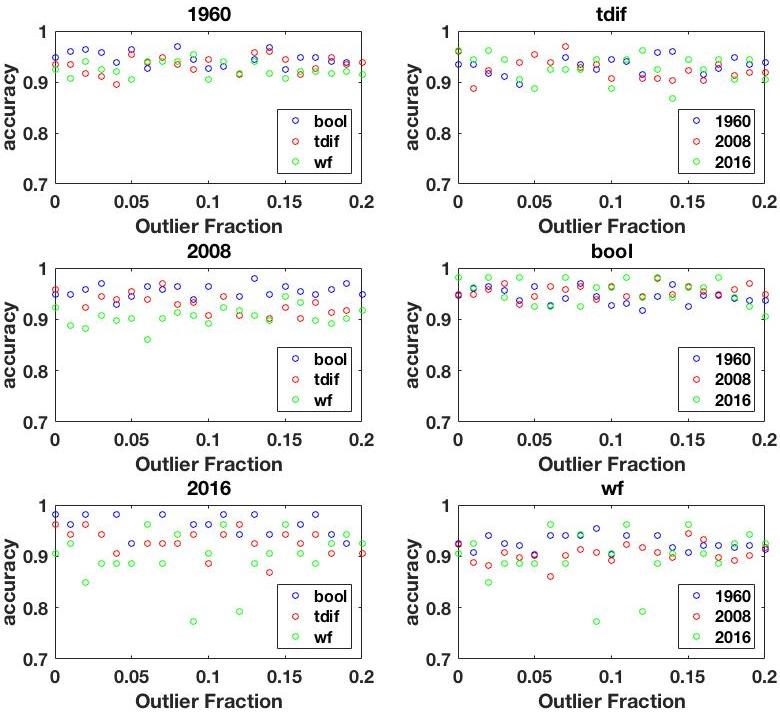
\includegraphics[width=.97\linewidth]{rsvm} 
\caption{Results from tuning the robust SVM implementation.}
\label{fig:svm}
\end{figure}
 
Another type of robust SVM implementation investigated here is described in \cite{xu}.  One could imagine defining a variable $\eta_i$ such that $0 \leq \eta_i \leq 1$ and $\eta_i = 0$ indicates that training element $i$ is an outlier. Naively, the robust problem could be as:
\begin{equation}
\min_\mathbf{w} \frac{\beta}{2} || \mathbf{w}||^2 + \sum_i \eta_i [1-y_i\mathbf{x}_i^\top\mathbf{w}]_+,
\end{equation}
so that outliers ($\eta_i = 0$) do not contribute to the loss function. Unfortunately, in this implementation the error $\eta_i [1-y_i\mathbf{x}_i^\top\mathbf{w}]_+$ is not an upper bound to the misclassification error. To remedy this, we add $1 - \eta_i$ to complete the robust hinge loss:
\begin{equation}
\eta \hbox{-} hinge(\mathbf{w}, \mathbf{x}, y) = \eta [1-y\mathbf{x}^\top\mathbf{w}]_+ + 1 - \eta.
\end{equation}
The new minimization problem is 
\begin{equation}
\min_{\substack{\mathbf{w} \\0\leq\eta_i\leq1}} \frac{\beta}{2} || \mathbf{w}||^2 + \sum_i \eta_i \hbox{-} hinge(\mathbf{w}, \mathbf{x}_i, y_i).
\end{equation}
The $\eta \hbox{-} hinge$ loss function further reduces to the robust loss function, described in \cite{krause, mason}:
\begin{equation}
robust(\mathbf{w}, \mathbf{x}, y) = min(1, hinge((\mathbf{w}, \mathbf{x}, y))).
\end{equation}
That is 
\begin{multline}
\min_{\substack{\mathbf{w} \\0\leq\eta_i\leq1}} \frac{\beta}{2} || \mathbf{w}||^2 + \sum_i \eta_i \hbox{-} hinge(\mathbf{w}, \mathbf{x}_i, y_i) \\
 = \min_{\mathbf{w}} \frac{\beta}{2} || \mathbf{w}||^2 + \sum_i robust(\mathbf{w}, \mathbf{x}_i, y_i)
\end{multline}

Due to time constraints, were were unable to finish implementing this method for our data; however, we would expect this robust SVM to perform better on moderate candidates that cross party lines. 

\subsection{KNN for text classification}

We investigate the applicability of a $k$-nearest neighbors classifier for speech recognition. While a naive Bayes classifier assumes that all words are independent features, a $k$-nearest neighbors algorithm allows us to classify speeches allowing for some degree of correlation between words in feature space. $k$-nearest neighbors algorithms have had some degree of success in the field of text classification, particularly when used to classify \textit{tfidf} data.

We define feature vectors by mapping each speech onto the entire list of 16,243 tokens. If a token does not appear in a speech, then the feature vector coordinate in the corresponding dimension is zero; if a token does appear in a speech, then the feature vector coordinate in the corresponding dimension is the frequency of the token, as defined by the relevant metric. We do not normalize or otherwise process these feature vectors in any way.

We train and test on values of $k$ ranging in integer steps from 1 to 25, and find that $k=1$ performs best for all trials with the exception of 2016 data, that tends to do better with higher $k$. This may be due to the fact that speeches given by the same candidate resemble each other much more than they resemble speeches given by other candidates; however, this may also be due to the lack of normalization favoring speeches of comparable length. The cross validation accuracy for each $k$ is shown in Figure \ref{fig:knn}.

\begin{figure}[t]
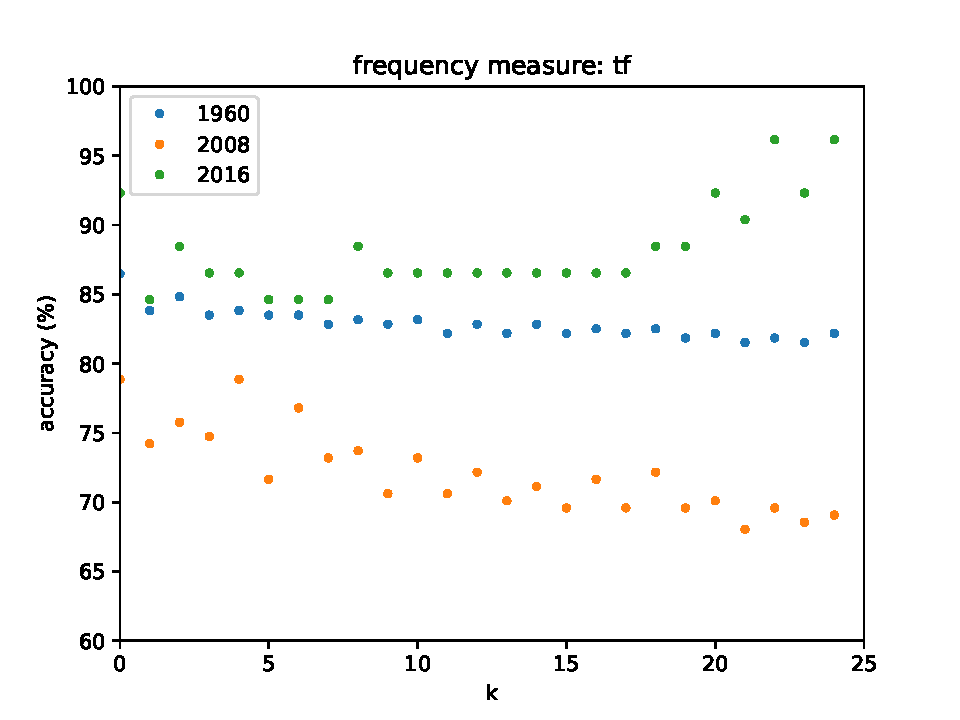
\includegraphics[width=.97\linewidth]{knn_tf} 
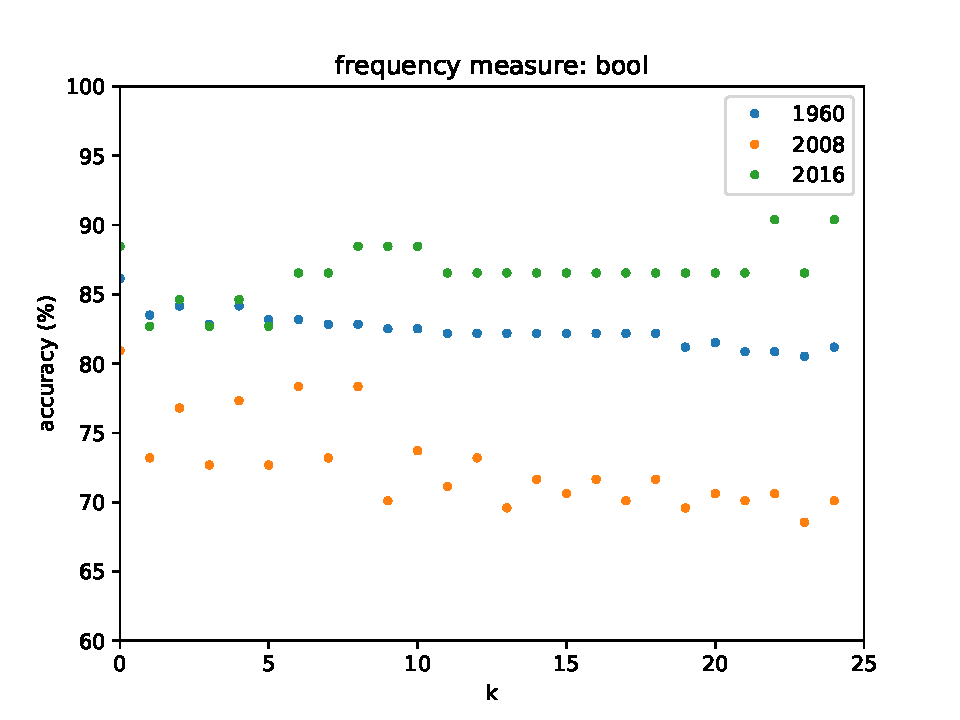
\includegraphics[width=.97\linewidth]{knn_bool} 
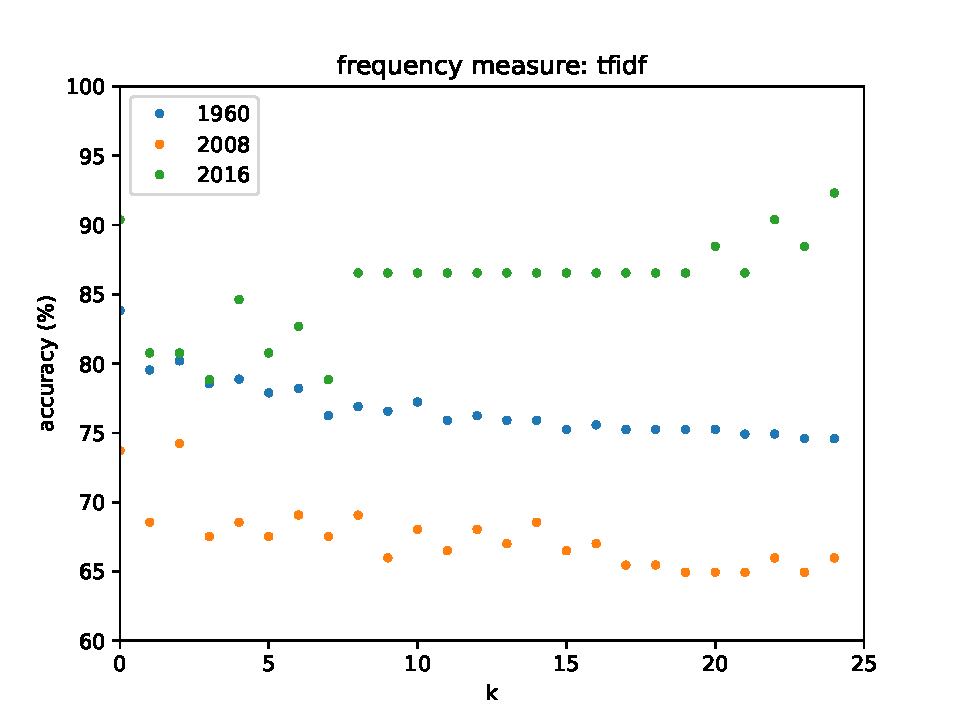
\includegraphics[width=.97\linewidth]{knn_tfidf} 
\caption{Training accuracy for each election cycle and word frequency measure. For the 1960 and 2008 election cycles $k\sim1$ performs best. For 2016, $k\sim25$ performs best.}
\label{fig:knn}
\end{figure}


%%% RESULTS %%%
\section{Results}

We use both cross validation and traditional training/testing to gain insights into partisanship in US campaigns for the 1960, 2008 and 2016 election cycles. We use cross validation within single election cycles to optimize model parameters (e.g. $C$ in SVM or $k$ in KNN). Comparing the cross validation scores between election cycles can give some insight into degree of polarization between parties; if parties are highly polarized, cross validation scores should be greater. We then train with data from one election cycle and test on the remaining two. This can quantify the degree to which party lines shift between election cycles. The results for each set of tests are summarized below. Note that the results for LR were simply produced with the \texttt{scikit} package \texttt{linear\_model.LinearRegression} as an early sanity check to ensure that the data was processed accurately. Similar tests were run with the \texttt{scikit} packages \texttt{naive\_bayes.MultinomialBayes} and \texttt{svm.LinearSVC} but the results are not reported here because the from-scratch NB and SVM modules we wrote perform comparable to or better than the early \texttt{scikit} tests.

\subsection{Cross validation}

The results for cross validating our classification methods within a single election cycle are shown in Table \ref{tab:crossval}. All classification methods perform adequately. KNN tends to do worse than other methods, especially for the 2008 campaign rhetoric, but does when using \textit{tfidf} word frequency. We expect that if the input feature vectors (texts) had been normalized, this classification may have improved.

The non-robust classification schemes (NB, SVM, and LR) perform best when trained and cross-validated on 1960 election data. We expect this is related to the fact that the 1960 election has the highest statistics, and only contains speeches from one speaker in each party (Nixon and Kennedy). That is, the classification schemes do well when they are comparing two people with different political leanings, but tend to do worse when given a selection of candidates in each party, as is the case in both 2008 and 2016. In other words, 1960 does not possess candidates that are ``outliers." We expected the classifiers to do better for election cycles that were generally considered to be more polarizing (like 2016) but the results are evidence that confounding factors (like number of speakers each in each category) prevent us from making a significant conclusion about party polarization over time. This would be an interesting area for further study and would likely require a larger sample of election years that could be split between years with a presidential incumbent or otherwise.

We also find that the boolean word frequency measure does best in cross validation tests for NB, SVM and LR. This emphasizes buzzwords that could be associated with a party but not used repeatedly throughout a speech. Surprisingly, the robust SVM does marginally worse than the standard SVM implementation. However we would need to increase the statistics of our tests to make any definitive conclusion.

\subsection{Predictions between years}

While we expect party values and talking points to evolve over time, we anticipate at least some predictive power when training on data from one election cycle and testing on another. Classification tends to do better when trained and tested on election cycles that are closer temporally. This is expected; the topics of interest change less between consecutive cycles than over the course of several decades. This is evident from the results in Table \ref{tab:results}, which confirms our belief that classifier accuracy worsens as party platforms and rhetorical style change. 2008 and 2016 are far better at predicting party affiliation in speeches between the two cycles than either is at predicting party affiliation in the 1960 election (though there are exceptions). In fact, when training on 1960 and testing on 2008/2016 and vice versa, we often to do worse than randomly guessing. This is reasonably consistent across classification schemes and word frequency metrics. We find that the most common misclassifications are 1960s Republicans being labeled as Democrat when trained with 2008 and 2016 data. The RSVM classifier is, again, comparable to the standard SVM.

\subsection{Predictive words}

The most predictive words for each party for each election cycle (and for all three combined) are shown in Table \ref{tab:words}. Particularly for the \textit{tf} and \textit{bool} frequency measures, the most common words strike a chord as the common sticking point for a particular election cycle. Though not listed, the fourth most indicative word for Democratic speech in 1960 was ``catholic"; Kennedy was the first Catholic president. Kennedy was also in the habit of listing prominent Republicans from the last century during his speeches, hence the indicative power of ``coolidg" (Calvin Coolidge, 30th President) and ``landon" (Alf Landon, 1936 Republican nominee). In 2008, race, of course, was a prominent topic, but so was economic strategy; ``trickle" (as in ``trickle-down economics," coined during the Reagan era) was a common word used by the Democrats to oppose large tax cuts to the wealthy. McCain commonly used the phrase ``shoulder a rifle" when expressing support for the troops --- he was a well-known war veteran himself. In 2016 multiple top words refer to wealth (``billionaire" and ``millionaire") and equality (``fairer" and ``ineq," the stem of words like ``inequality"). There's an indirect reference to Clinton's emails (``delet" --- this was a common talking point for Trump). And healthcare made the top contenders in 2016 as well: ``obamacar" was indicative of Republican speech (it was yet another common talking point for Trump). These words provide a unique lens into the politics of the era and are interesting in their own right. We see signs of the most prominent social, economic, and political issues during each election period.

\begin{table} % use table* for two-column table
  \begin{ruledtabular}
  %  \newcommand{\twrw}[1]{\multirow{2}{*}{#1}}
  \begin{tabular}{ccccc}
  Method & Freq.& 1960 & 2008 & 2016 \\
    \hline
 & \textit{tf} & 97.4  & 90.7 & 94.2 \\
NB & \textit{bool} & 95.0  & 90.7 & 98.1 \\
 & \textit{tfidf} & 97.4  & 93.3 & 92.3 \\
 \hline
 & \textit{tf} & 94.1 & 91.8 & 90.6 \\
SVM & \textit{bool} & 96.7 & 98.0 & 94.3 \\
 & \textit{tfidf} & 94.4 & 91.3 & 88.7 \\
 \hline
   & \textit{tf} & 89.8  & 88.2 & 85.6 \\
LR (\texttt{scikit}) & \textit{bool} & 93.3  & 92.9 & 91.2 \\
 & \textit{tfidf} & 90.1  & 88.3 & 89.3 \\
 \hline
   & \textit{tf} & 86.5  & 78.9 & 92.3 \\
KNN & \textit{bool} & 86.1  & 80.9 & 88.5 \\ 
 & \textit{tfidf} & 83.8  & 73.7 & 90.4 \\
 \hline
  & \textit{tf} & 90.4  & 90.3 & 88.7 \\
RSVM & \textit{bool} & 96.4  & 94.4 & 92.5 \\
 & \textit{tfidf} & 95.4  & 95.4 & 88.7 \\
 \hline
  \end{tabular}
  \end{ruledtabular}
    \caption{Cross validation scores by method and word frequency metric.}
     \label{tab:crossval}
\end{table}

\begin{table*} % use table* for two-column table
  \begin{ruledtabular}
  %  \newcommand{\twrw}[1]{\multirow{2}{*}{#1}}
  \begin{tabular}{ccccc}
   Method & Training Year & 1960 (\textit{tf}/\textit{bool}/\textit{tfidf}) & 2008 (\textit{tf}/\textit{bool}/\textit{tfidf}) & 2016 (\textit{tf}/\textit{bool}/\textit{tfidf}) \\
    \hline
 & 1960 & ---  & 45.4/\textit{39.2}/\textit{38.7} & 50.0/51.9/50.0 \\
NB & 2008 & \textit{41.6}/\textbf{60.7}/55.4  & --- & \textbf{76.9}/53.8/57.7 \\
 & 2016 & \textbf{65.0}/\textbf{66.0}/\textbf{65.3}  & \textbf{63.4}/\textbf{64.9}/\textbf{62.4} & --- \\
 \hline
  & 1960 & ---  & \textit{40.2}/\textit{44.7}/\textit{40.1} & 55.1/\textit{40.5}/52.5 \\
SVM & 2008 & \textit{37.3}/56.9/\textit{40.7}  & --- & \textbf{70.3}/55.1/\textbf{63.9} \\
 & 2016 & \textit{59.3}/58.4/\textbf{64.0}  & \textbf{72.4}/\textbf{66.3}/\textbf{63.5} & --- \\
 \hline
  & 1960 & ---  & 47.1/51.0/48.3 & 54.1/47.1/55.4 \\
LR & 2008 & \textit{41.3}/47.1/\textit{44.4}  & --- & \textbf{66.2}/59.2/50.3 \\
 & 2016 & 51.8/55.9/51.5  & \textbf{67.1}/\textbf{67.8}/\textbf{71.2} & --- \\
 \hline
  & 1960 & ---  & \textit{43.8}/49.0/55.2 & \textit{28.8}/50.0/\textit{38.5} \\
KNN & 2008 & 59.4/\textbf{62.0}/\textbf{65.0}  & --- & 53.8/50.0/\textit{44.2} \\
 & 2016 & \textit{22.1}/\textit{28.0}/\textit{33.0}  & \textbf{68.0}/\textbf{63.9}/53.6 & --- \\
 \hline
  & 1960 & ---  & \textit{42.0}/53.3/\textit{40.4} & 46.2/\textit{43.7}/\textit{44.9} \\
RSVM & 2008 & \textit{33.8}/51.4/\textit{39.4}  & --- & 58.9/\textbf{66.5}/51.3 \\
 & 2016 & \textit{40.0}/56.7/\textit{34.4}  & \textbf{71.8}/\textbf{64.7}/\textbf{70.4} & --- \\
 \hline
  \end{tabular}
  \end{ruledtabular}
    \caption{The accuracies for training on one election year and testing on another election year where we have emphasized testing accuracies $\mathbf{> 60\%}$ and $\mathit{< 45\%}$. The cross-year training/testing tends to do better on years that are closer in time.}
     \label{tab:results}
\end{table*}

\begin{table*} % use table* for two-column table
  \begin{ruledtabular}
  %  \newcommand{\twrw}[1]{\multirow{2}{*}{#1}}
  \begin{tabular}{cccc}
  Year & Freq. & Democrat & Republican \\
    \hline
 & \textit{tf} & coolidg, landon, forsight  & incident, standpoint, surrend   \\
1960 & \textit{bool} & coolidg, landon, forsight   & incident, standpoint, tear  \\
 & \textit{tfidf} & dribble, cold, blackwel  & hanov, corrobor, conced  \\
 \hline
 & \textit{tf} & dime, trickl, racial  & brokaw, constru, jihadist  \\
2008 & \textit{bool} & dime, trickl, workplac  & rifl, despis, discretionari  \\
 & \textit{tfidf} & bricklay, highli, jindal  & assuage, dispatch, best  \\
 \hline
 & \textit{tf} & billionair, wealthiest, vermont  & obamacar, renegoti, delet   \\
2016 & \textit{bool} & billionair, fairer, ineq   & delet, renegoti, salut    \\
 & \textit{tfidf} & bad, quito, protest    & machin, outlcass, conspicu   \\
 \hline
  & \textit{tf} & billionare, coolidg, landon   & standpoint, obamacar, incident  \\
combined & \textit{bool} & coolidg, billionare, landon   & standpoint, delet, incident  \\
 & \textit{tfidf} & alumnu, avert, compulsori  & animos, downplay, barren  \\
 \hline
  \end{tabular}
  \end{ruledtabular}
    \caption{The words most indicative of both political parties based on election year and word frequency metric.}
    \label{tab:words}
\end{table*}


%%% CONCLUSIONS %%%
\section{Conclusions}

We found that each of the classification methods we tested was able to predict party affiliation when constrained to a single election cycle. Election cycles that are close together in time (e.g. 2008 and 2016) have some predictive power when trained on one and tested on the other. However, the predictive power breaks down as election cycles move further apart. When training on 2008 and 2016 election cycles, the predictions often classified 1960 Republican speeches as Democrat speech. Further study could be done to expand the dataset to examine the change of rhetoric from year to year and explore how long a particular election cycle might be predictive for future election cycles. Ideally a full corpora containing each election cycle could be used to make further conclusions. However, one would need to consider that a confounding factor may be the presence or absence of an incumbent running in the election for a particular year. This candidate would have no opponent within their own party and may speak differently as a result.

We explored the use of robust support vector machines to better classify moderate candidates whose speech can jump across party lines. Existing literature has shown that the standard SVM classifier performs worse on floor speeches from the more partisan House than in the Senate. We found that the RSVM did not significantly improve our ability to classify data, but we are unable to make statistically significant conclusions given the data. We expect that further study would elucidate the advantages or disadvantages of using a RSVM method to reduce the impact of outliers.

%%% MEMBER CONTRIBUTIONS %%%
\section{Member contributions}

Julia was responsible for implementing our SVM and robust SVM classifiers. She drafted the related text in this document (with additional contributions throughout the text during the editing process) and studied a great deal of possible robust implementations while working on this project before settling on the final result. Garrett produced the NB and KNN results along with the corresponding text in this paper (with additional contributions throughout the text during editing). He initially planned to implement a robust version of NB, but found that it was best suited for anomaly detection rather than the type of outlier robusticity we sought. Rory was responsible for data acquisition, processing, and initial testing with \texttt{scikit} packages to ensure the project was viable. She compiled all results in the first full draft of this report.

\begin{thebibliography}{7}

\bibitem{chandra}
Chandra, B. \textit{et. al.} (2007). Robust Approach for Estimating Probabilities in Naive-Bayes Classifier. \textit{International Conference on Pattern Recognition and Machine Intelligence}, 11-16.

\bibitem{kwon}
Kwon, N. \textit{et. al.} (2006). Identifying and classifying subjective claims. \textit{Proceedings of the 8th Annual International Digital Government Research Conference}, 76-��81.

\bibitem{mccallum}
McCallum, A. \& Nigam, K. (1998). A comparison of event models for naive Bayes text classification. \textit{Proceedings of the 1998 Association for the Advancement of Artificial Intelligence Workshop on Learning for Text Categorization (AAAI’98)}, 41�-48.

\bibitem{peters}
Peters, G.,The American Presidency Project [online]. Santa Barbara, CA: University of California (hosted), Gerhard Peters (database). Available from World Wide Web: http://www.presidency.ucsb.edu/

\bibitem{thomas}
Thomas, M. \textit{et. al.} (2006). Get out the vote: Determining support or opposition from Congressional floor-debate transcripts. \textit{Proceedings of the 2006 Conference on Empirical Methods in Natural Language Processing (EMNLP’06)}, 327-��335.

\bibitem{xu}
Xu, L. \textit{et. al.} (2006). Robust Support Vector Machine Training via Convex Outlier Ablation. \textit{Proceedings of the 21st national conference on Artificial intelligence}, Vol 1, 536-542.

\bibitem{yu}
Yu, B. \textit{et. al.} (2008). Classifying party affiliation from political speech. \textit{Journal of Information Technology \& Politics}, 5:1, 33-48, DOI: 10.1080/19331680802149608

\bibitem{krause}
Krause, N., \& Singer, Y. (2004). Leveraging the margin more carefully. \textit{Proceedings ICML}.

\bibitem{mason}
Mason, L. \textit{et. al.} (2000). Functional gradient techniques for combining hypotheses. \textit{Advances in Large Margin Classifiers}. MIT Press.

\bibitem{Kecman}
Kecman, V., Han T.M., and Vogt, M. (2006). Iterative Single Data Algorithm for Training Kernel Machines from Huge Data Sets: Theory and Performance. \textit{Kernel Based Algorithms for Mining Huge Data Sets. Studies in Computational Intelligence vol 17}. Springer, Berlin, Heidelberg.

\end{thebibliography}

\end{document}





